\refstepcounter{appendixctr}\label{hwansappendix}%
\appendix\chapter{Appendix \ref{hwansappendix}: Hints and Solutions}


%==================================================================
%==================================================================
%========================= Hints ==================================
%==================================================================
%==================================================================

\noindent\formatlikesection{Hints}

\noindent\formatlikesubsection{Hints for Chapter \ref{ch:2}}\\
\hwanshdr{atwood-energy-sn}\label{hwhint:atwood-energy-sn} You can use either
the chain-rule technique from page  \pageref{gaccelproof} or the technique prescribed
in problem \ref{hw:gaccelproof2} on p. \pageref{hw:gaccelproof2}. The
positions and velocities of the two masses are related to each other, and you'll need
to use this relationship to eliminate one mass's position and velocity and get everything
in terms of the other mass's position and velocity. The relationship between the
two positions will involve some extraneous variables like the length of the string,
which won't have any effect on your final result.

\hwanshdr{pulley}\label{hwhint:pulley} This is similar to problem \ref{hw:atwood-energy-sn},
but you're trying to find the combination of masses that will result in \emph{zero}
acceleration. In this problem, the distance dropped
by one weight is different from, but still related to,
 the distance by which the other weight rises. Try relating the heights of the
 two weights to each other, so you can get the total gravitational energy in terms
 of only one of these heights.
 
\hwanshdr{tightropish}\label{hwhint:tightropish} This is similar to problem
\ref{hw:pulley}, in that you're looking for a setup that will give zero
acceleration, and the distance the middle weight rises or falls is not the same as the distance
the other two weights fall or rise. The simplest approach is to get the three heights
in terms of $\theta$, so that you can write the gravitational energy in terms of $\theta$.

\hwanshdr{funkyatwood}\label{hwhint:funkyatwood} This is very similar to problems
\ref{hw:atwood-energy-sn} and \ref{hw:pulley}.

\hwanshdr{lennardjones}\label{hwhint:lennardjones} The first two parts can be done more easily by
setting $a=1$, since the value of $a$ only changes the distance
scale.

\hwanshdr{geosynch}\label{hwhint:geosynch} The condition for a circular orbit
contains three unknowns, $v$, $g$, and $r$, so you can't just solve it for $r$. You'll need
more equations to make three equations in three unknowns. You'll need a relationship
between $g$ and $r$, and also a relationship between $v$ and $r$ that uses the
given fact that it's supposed to take 24 hours for an orbit.

\hwanshdr{escape2}\label{hwhint:escape2} What does the total energy have to
be if the projectile's velocity is exactly escape velocity? Write down conservation
of energy, change $v$ to $\der{}r/\der{}t$, separate the variables, and integrate.

\hwanshdr{tides}\label{hwhint:tides} The analytic approach is a little cumbersome,
although it can be done  by using approximations like
$1/\sqrt{1+\epsilon}\approx1-(1/2)\epsilon$. A more straightforward, brute-force
method is simply to write a computer program that calculates $U/m$ for
a given point in spherical coordinates. By trial and error, you can fairly rapidly
find the $r$ that gives a desired value of $U/m$.

\hwanshdr{hangfromspring}\label{hwhint:hangfromspring}
Use calculus to find the minimum of $U$.

\hwanshdr{pulleyandspring}\label{hwhint:pulleyandspring}
The spring constant of this spring, $k$, is \emph{not} the quantity
you need in the equation for the period. What you need in that equation
is the second derivative of the spring's energy with respect to the
position of the thing that's oscillating. You need to 
start by finding the energy stored in the spring as a function of
the vertical position, $y$, of the mass. This is similar to
example \ref{eg:leverspring} on page \pageref{eg:leverspring}.

\hwanshdr{springsseries}\label{hwhint:springsseries} The variables
$x_1$ and $x_2$ will adjust themselves to reach an equilibrium. Write down the total
energy in terms of $x_1$ and $x_2$, then eliminate one variable, and find the
equilibrium value of the other. Finally, eliminate both $x_1$ and $x_2$ from the
total energy, getting it just in terms of $b$.


\noindent\formatlikesubsection{Hints for Chapter \ref{ch:3}}\\
\hwanshdr{tugboat}\label{hwhint:tugboat} Write down two equations, one for Newton's
	second law applied to each object. Solve these for the two
	unknowns $T$ and $a$.
	
\hwanshdr{maxampatdc}\label{hwhint:maxampatdc}
The whole expression for the amplitude has maxima where the
stuff inside the square root is at a minimum, and vice versa, so
you can save yourself a lot of work by just working on the stuff
inside the square root. For normal, large values of $Q$, the
there are two extrema, one at $\omega=0$ and one at
resonance; one of these is a maximum and one is a minimum.
You want to find out at what value of $Q$ the zero-frequency extremum
switches over from being a maximum to being a minimum.

\hwanshdr{anglebetween}\label{hwhint:anglebetween}
You can use the geometric interpretation of the dot product.

\hwanshdr{ropeslopes}\label{hwhint:ropeslopes}
The easiest way to do this problem is to use two different coordinate
systems: one that's tilted to coincide with the upper slope, and one that's
tilted to coincide with the lower one.

\noindent\formatlikesubsection{Hints for Chapter \ref{ch:4}}\\
\hwanshdr{tipbox}\label{hwhint:tipbox}
The choice of axis theorem only applies to a closed system, or to a
system acted on by a total force of zero. Even if the box is not going
to rotate, its center of mass is going to accelerate,
and this can still cause a change in its angular momentum, unless
the right axis is chosen. For example, if the axis is chosen
at the bottom right corner, then the box will start accumulating
clockwise angular momentum, even if it is just accelerating to the
right without rotating. Only by choosing the axis at the center of
mass (or at some other point on the same horizontal line) do we get
a constant, zero angular momentum.

\hwanshdr{wheeloverstep}\label{hwhint:wheeloverstep}
There are four
forces on the wheel at first, but only three when it lifts
off. Normal forces are always perpendicular to the surface
of contact. Note that the corner of the step cannot be
perfectly sharp, so the surface of contact for this force
really coincides with the surface of the wheel.

\hwanshdr{tetherball}\label{hwhint:tetherball}
How is this different
from the case where you whirl a rock in a circle on a string
and gradually pull in the string?


\hwanshdr{yoyo}\label{hwhint:yoyo}
The acceleration and the tension in the string are unknown.
Use $\tau=\der L/\der t$ and $F=ma$ to determine these two unknowns.


\hwanshdr{erbium}\label{hwhint:erbium}
You'll need the result of problem \ref{hw:anganalogies} in order
to relate the energy and angular momentum of a rigidly rotating body.
Since this relationship involves a variable raised to a power,
you can't just graph the data and get the moment of inertia
directly. One way to get around this is to
manipulate one of the variables to make the graph linear.
Here is an example of this technique from
another context. Suppose you were given a table of the masses, $m$, of cubical
pieces of wood, whose sides had various lengths, $b$. You want
to find a best-fit value for the density of the wood.
The relationship is $m=\rho b^3$. The graph of $m$ versus $b$ would be a curve,
and you would not have any easy way to get the density from such
a graph. But by graphing $m$ versus $b^3$, you can produce a graph that
is linear, and whose slope equals the density.

\noindent\formatlikesubsection{Hints for Chapter \ref{ch:waves}}\\
\hwanshdr{sinwavekinem}\label{hwhint:sinwavekinem}
How could you change the values of $x$ and $t$ so that the value of
$y$ would remain the same? What would this represent physically?

\hwanshdr{airwaterrefl}\label{hwhint:airwaterrefl}
The answers to the two parts are not the same.

\hwanshdr{lasso}\label{hwhint:lasso}
(a) The most straightforward approach is to apply the
equation $\partial^2y/\partial t^2=(T/\mu)\partial^2y/\partial x^2$.
Although this equation was developed in the main text in the
context of a straight string with a curvy wave on it, it works just
as well for a circular loop; the left-hand side is simply the inward
acceleration of any point on the rope. Note, however, that we've been
assuming the string was (at least approximately) parallel to the $x$ axis,
which will only be true if you choose a specific value of $x$.
You need to get an equation for
$y$ in terms of $x$ in order to evaluate the right-hand side.

\noindent\formatlikesubsection{Hints for Chapter \ref{ch:rel}}\\
\hwanshdr{tossed-clock}\label{hwhint:tossed-clock}
 Apply the equivalence principle.


\noindent\formatlikesubsection{Hints for Chapter \ref{ch:atomem}}\\
\hwanshdr{nacl}\label{hwhint:nacl}
The force
on the lithium ion is the vector sum of all the forces of
all the quadrillions of sodium and chlorine atoms, which
would obviously be too laborious to calculate.  Nearly all
of these forces, however, are canceled by a force from an
ion on the opposite side of the lithium.



\noindent\formatlikesubsection{Hints for Chapter \ref{ch:efield}}\\
\hwanshdr{dipolev}\label{hwhint:dipolev}
Use the approximation $(1+\epsilon)^p\approx1+p\epsilon$, 
which is valid for small $\epsilon$.

\hwanshdr{vedgedisk}\label{hwhint:vedgedisk}
The math is messy if you put the origin of your polar coordinates
at the center of the disk. It comes out much simpler
if you put the origin at the edge, right on top of the point at
which we're trying to compute the voltage.

\hwanshdr{neuronenergy}\label{hwhint:neuronenergy}
Since we have $t\ll r$, the volume of the membrane is essentially
the same as if it was unrolled and flattened out, and the
field's magnitude is nearly constant.

\hwanshdr{epointinfty}\label{hwhint:epointinfty}
First find the energy stored in a spherical shell extending
from $r$ to $r+\der r$, then integrate to find the total
energy.

\noindent\formatlikesubsection{Hints for Chapter \ref{ch:em}}\\
\hwanshdr{nestedsolenoids}\label{hwhint:nestedsolenoids}
A stable system has low energy; energy would have to be added to
change its configuration.

\hwanshdr{solarconstant}\label{hwhint:solarconstant}
We're ignoring the fact that the light consists of little
wavepackets, and imagining it as a simple sine wave. But wait, there's
more good news! The energy density depends on the squares of the fields,
which means the squares of some sine waves. Well, when you square a sine
wave that varies from $-1$ to $+1$, you get a sine wave that goes from
0 to $+1$, and the average value of that sine wave is 1/2. That means
you don't have to do an integral like $U=\int (\der U/\der V)\der V$.
All you have to do is throw in the appropriate factor of 1/2, and you
can pretend that the fields have their constant values
$\tilde{\vc{E}}$ and $\tilde{\vc{B}}$ everywhere.


\hwanshdr{circularcap}\label{hwhint:circularcap}
Use Faraday's law, and choose an Amp\`{e}rian surface that
is a disk of radius $R$ sandwiched between the plates.

\hwanshdr{timereversalem}\label{hwhint:timereversalem}
(a) Magnetic fields are created by currents, so once you've
decided how currents behave under time-reversal, you can
figure out how magnetic fields behave.
	
\noindent\formatlikesubsection{Hints for Chapter \ref{ch:optics}}\\
\hwanshdr{very-weak-refraction}\label{hwhint:very-weak-refraction}
Expand $\sin\theta$ in a Taylor series around $\theta=90\ \degunit$.


	
	
%==================================================================
%==================================================================
%========================= Self-Checks ============================
%==================================================================
%==================================================================




\noindent\formatlikesection{Answers to Self-Checks}


\noindent\formatlikesubsection{Answers to Self-Checks for Chapter \ref{ch:intro}}\\

\scanshdr{psychic}
If only he has the special powers, then his results can never be
reproduced.

\scanshdr{cathode-rays}
They would have had to weigh the rays, or check for a loss of weight  in
 the object from which they were have
emitted.  (For technical reasons, this was not a measurement
 they could actually do, hence the opportunity for
disagreement.)

\scanshdr{operational-definition}
A dictionary might define ``strong'' as ``possessing powerful muscles,''
but that's not an operational definition, because
it doesn't say how to measure strength numerically. 
 One possible operational definition would be the number of
pounds a person can bench press.

\scanshdr{slow-time}
A microsecond is 1000 times longer than a nanosecond, so it would seem like 1000 seconds, or about 20 minutes.

\scanshdr{bacteria-queue}
Exponents have to do with multiplication, not addition. The
first line should be 100 times longer than the second,
not just twice as long.

\scanshdr{nigeria}
The various estimates differ by 5 to 10 million. The
CIA's estimate includes a ridiculous number of gratuitous
significant figures. Does the CIA understand that every
day, people in are born in, die in,  immigrate to, and
emigrate from Nigeria?

\scanshdr{count-sig-figs}
(1) 4; (2) 2; (3) 2

\scanshdr{yd2-yd3}
$1\ \zu{yd}^2\times(3\ \zu{ft}/1\ \zu{yd})^2=9\ \zu{ft}^2$\\
$1\ \zu{yd}^3\times(3\ \zu{ft}/1\ \zu{yd})^3=27\ \zu{ft}^3$

\scanshdr{axle-ratios}
$C_1/C_2=(w_1/w_2)^4$


\noindent\formatlikesubsection{Answers to Self-Checks for Chapter \ref{ch:1}}\\
\scanshdr{hoseup} The stream has to spread out. When the velocity becomes zero,
it seems like the cross-sectional area has to become infinite. In reality, this is the point
where the water turns around and comes back down. The infinity isn't real; it occurs
mathematically because we used a simplified model of the the stream of water, assuming,
for instance, that the water's velocity is always straight up.\\
\scanshdr{dxsign} A positive $\Delta x$ means the object is moving in the same
direction as the positive $x$ axis. A negative $\Delta x$ means it's going the opposite
direction.\\
\scanshdr{inertia-counterexamples}
(1) The effect only occurs during blastoff, when their velocity is changing. Once
 the rocket engines stop firing, their
velocity stops changing, and they no longer feel any effect. (2) It
 is only an observable effect of your motion relative
to the air.\\
\scanshdr{beer}Galilean relativity says that experiments can't come out differently
just because they're performed while in motion. The tilting of the surface tells us the
train is accelerating, but it doesn't tell us anything about the train's velocity at that
instant. The person in the train might say the bottle's velocity was zero (but changing),
whereas a person
working in a reference frame attached to the dirt outside says it's moving; they don't
agree on velocities. They \emph{do} agree on accelerations. The person in the train
has to agree that the train is accelerating, since otherwise there's no reason for the
funny tilting effect. \\
\scanshdr{moneyquantum}Yes. In U.S. currency, for instance, the quantum of money
is one cent.\\

\noindent\formatlikesubsection{Answers to Self-Checks for Chapter \ref{ch:2}}\\
\scanshdr{cardiag}
There are two reasonable possibilities we could imagine --- neither of which ends
up making much sense --- if we insist on the straight-line trajectory.
(1) If the car has constant speed along the line, then in the * frame we see it
going straight down at constant speed. It makes sense that it goes straight down
in the * frame of reference, since in that frame it was
never moving horizontally, and there's no reason for it to start. However, it
doesn't make sense that it goes down with constant speed, since falling objects
are supposed to speed up the whole time they fall. This violates both Galilean
relativity and conservation of energy.
(2) If it's speeding up and moving along a diagonal line in the
original frame, then it might be conserving energy in one frame or the other.
But if it's speeding up along a line, then as seen in the original frame, both 
its vertical motion and its horizontal motion must be speeding up.
If its horizontal velocity is increasing in the original frame, then it can't be zero
and remain zero in the * frame. This violates Galilean relativity, since in the *
frame the car apparently starts moving sideways for no reason.

\noindent\formatlikesubsection{Answers to Self-Checks for Chapter \ref{ch:3}}\\
\scanshdr{gymnastics-wheel}
By shifting his weight around, he can cause the center of mass not to coincide
with the geometric center of whe wheel.

\scanshdr{force-or-not}
(1) This is motion, not force. (2) This is a description of how the
 sub is able to get the water to produce a forward
force on it. (3) The sub runs out of energy, not force.

\scanshdr{static-or-kinetic}
(1) It's kinetic friction, because her uniform is sliding over
 the dirt. (2) It's static friction, because even though the
two surfaces are moving relative to the landscape, they're not slipping
 over each other. (3) Only kinetic friction
creates heat, as when you rub your hands together. If you
 move your hands up and down together without sliding
them across each other, no heat is produced by the static friction.


\scanshdr{frictionnormal}Frictionless (or nearly frictionless) ice can certainly make
a normal force, since otherwise a hockey puck would sink into the ice. Friction
is not possible without a normal force, however: we can see this from the equation,
or from common sense, e.g. while sliding down a rope you don't get any friction
unless you grip the rope.

\scanshdr{find-directions-of-forces}
(1) Normal forces are always perpendicular to the surface of contact,
 which means right or left in this figure. Normal
forces are repulsive, so the cliff's force on the feet
 is to the right, i.e., away from the cliff.  (2) Frictional forces are
always parallel to the surface of contact, which means right or left
 in this figure. Static frictional forces are in the
direction that would tend to keep the surfaces from slipping over
 each other. If the wheel was going to slip, its
surface would be moving to the left, so the static frictional force on
 the wheel must be in the direction that would
prevent this, i.e., to the right. This makes sense, because it is
 the static frictional force that accelerates the
dragster.  (3) Normal forces are always perpendicular to the surface of
 contact. In this diagram, that means either
up and to the left or down and to the right. Normal forces are 
repulsive, so the ball is pushing the bat away from
itself. Therefore the ball's force is down and to the right on this diagram.

\scanshdr{swing-energy}
The dashed lines on the graph are about twice as far apart in the second cycle compared
to the first, so the amplitude has doubled. For sufficiently small oscillations around an equilibrium
with $x=0$ and $U(0)=0$, it's always a good approximation to take $U\propto x^2$, so the energy
is proportional to the square of the amplitude; this is a general fact about all oscillations,
provided that the amplitude is small. Since the amplitude doubled, the energy quadrupled.

\scanshdr{compare-damping}
The two graphs start off with the same amplitude, but the solid curve loses
amplitude more rapidly. For a given time, $t$, the quantity $e^{-ct}$ is apparently
smaller for the solid curve, meaning that $ct$ is greater. The solid curve has
the higher value of $c$.

\scanshdr{q-is-when-dead}
A decaying exponential never dies out to zero in any finite amount of time.

\scanshdr{a-propto-q}
In the expression 
\begin{equation*}
		A = 
			= \frac{F_m}{m\sqrt{\left(\omega^2-\omega_\zu{o}^2\right)^2
				+\omega_\zu{o}^2\omega^2Q^{-2}}}
\end{equation*}
from page \pageref{resonance-amplitude}, substituting $\omega=\omega_\zu{o}$ makes the first
term inside the square root vanish, which should make the denominator pretty small, thereby
producing a pretty big amplitude. In the limit of $Q=\infty$, $Q^{-2}=0$, so the second term
vanishes, and $\omega=\omega_\zu{o}$ actually produces an infinite amplitude. For values of $Q$
that are large but finite, we still expect to get resonance pretty close to $\omega=\omega_\zu{o}$.
Setting $\omega=\omega_\zu{o}$ in the finite-$Q$ case, the first
term vanishes, we can simplify the square root, and the result ends up being $A\propto 1/\sqrt{Q^{-2}}\propto Q$.
This is only an approximation, because we had to assume early on that $Q$ was large.

\scanshdr{translatefvector} $\zb{F}=m\zb{a}$

\scanshdr{graphicalscalarmult} \\
\begin{center}\anonymousinlinefig{graphicalscalarmultans}\end{center}

\noindent\formatlikesubsection{Answers to Self-Checks for Chapter \ref{ch:4}}\\
\scanshdr{torque} Torques 1, 2, and 4 all have the same sign, because they are trying to twist the wrench clockwise. The sign of 3 is opposite to the signs of 1, 2, and 4. The magnitude of 3 is the greatest, since it has a large $r$ and the force is nearly all perpendicular to the wrench. Torques 1 and 2 are the same because they have the same values of $r$ and $F_{\perp}$. Torque 4 is the smallest, due to its small $r$.

\scanshdr{thetazero} One person's $\theta$-$t$ graph would simply be shifted up or
down relative to the others. The derivative equals the slope of the tangent line,
and this slope isn't changed when you shift the graph, so both people would agree
on the angular velocity.

\scanshdr{omegasigns} Reversing the direction of $\omega$ also reverses the direction of 
motion, and this is reflected by the relationship between the plus and minus signs.
 In the equation for the radial acceleration, $\omega$ is squared, so even if $\omega$
 is negative, the
 result is positive. This makes sense because the acceleration is always inward in
 circular motion, never outward.

\scanshdr{righthanddtheta} All the rotations around the $x$ axis give $\omega$ vectors 
along the positive $x$ axis (thumb pointing along positive $x$), and all the rotations about 
the $y$ axis have $\omega$ vectors with positive $y$ components.

\scanshdr{anticommutative} For example, if we take
 $(\zb{A}\times\zb{B})_x=  A_yB_z - B_yA_z$ and reverse the A's and B's, we
get $(\zb{B}\times\zb{A})_x=  B_yA_z - A_yB_z$, which is just the negative of
the original expression.

\noindent\formatlikesubsection{Answers to Self-Checks for Chapter \ref{ch:thermo}}\\
\scanshdr{solidspressureside} Solids can exert shear forces. A solid could be
in an equilibrium in which the shear forces were canceling the forces due to
sideways pressure gradients. For example, if I push on a brick wall, it will give by
perhaps a millionth of an inch, but it will reach an equilibrium, in which the shear forces
cancel out the effect of the pressure gradient.

\scanshdr{pressureconst} (1) Not valid. The equation only applies to fluids. (2)
Valid. The density of the air is nearly constant between the
top and bottom of the building. (3) Not valid. There is a
large difference is the density of the air between the top
and the bottom of the mountain. (4) Not valid, because $g$
isn't constant throughout the interior of the earth. (5) Not
valid, because the air is flowing around the wing. The air
is accelerating, so it is not in equilibrium.

\scanshdr{idealgasentropy} Heating the gas at constant pressure requires
adding heat to it, which increases its entropy. To increase the gas's pressure
while keeping its temperature constant, we would have to compress it,
which would give it a smaller volume to inhabit, and therefore fewer possible
positions for each atom. The whole thing has to be proportional to $n$ because
entropy is additive.


\noindent\formatlikesubsection{Answers to Self-Checks for Chapter \ref{ch:waves}}\\
\scanshdr{coilspringvel} The leading edge is moving up, the trailing edge is moving
down, and the top of the hump is motionless for one instant.

\scanshdr{reflenergy} The energy of a wave is usually proportional
to the square of the amplitude. Squaring a negative number
gives a positive result, so the energy is the same

\scanshdr{sonarinvisibility} A substance is invisible to sonar if the speed of sound
waves in it is the same as  in water. Reflections occur only
at boundaries between media in which the wave speed is
different.

\scanshdr{wavelosesnergy} No. A material object that loses kinetic energy slows down,
but a wave is not a material object. The velocity of a wave
ordinarily only depends on the medium, not on the amplitude.
The speed of soft sound, for example,  is the same as the
speed of loud sound.

\scanshdr{perfectopticalcoating} No. To get the best possible interference, the thickness of
the coating must be such that the second reflected wave
train lags behind the first by an integer number of
wavelengths. Optimal performance can therefore only be
produced for one specific color of light. The typical
greenish color of the coatings shows that it does the worst
job for green light.

\scanshdr{passtwice} The period is the
time required to travel a distance $2L$ at speed $v$, $T=2L/v$.
The frequency is $f=1/T=v/2L$.

\scanshdr{asymmpipemodes} The wave pattern
will look like this:   
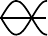
\includegraphics{\chapdir/figs/threequarterwave}
Three quarters of a wavelength fit
in the tube, so the wavelength is three times shorter than
that of the lowest-frequency mode, in which one quarter of a
wave fits. Since the wavelength is smaller by a factor of
three, the frequency is three times higher. Instead of
$f_\zu{o},\ 2f_\zu{o},\ 3f_\zu{o},\ 4f_\zu{o},\ \ldots$, the pattern of wave frequencies of this
air column goes $f_\zu{o},\ 3f_\zu{o},\ 5f_\zu{o},\ 7f_\zu{o},\ \ldots$


\noindent\formatlikesubsection{Answers to Self-Checks for Chapter \ref{ch:rel}}\\
\scanshdr{gammaatvzero} At $v=0$, we get $\gamma=1$, so $t=T$. There is
no time distortion unless the two frames of reference are in relative motion.

\scanshdr{unequalcollisioncons} The total momentum is zero before the collision. After the
collision, the two momenta have reversed their directions, but they still cancel.
Neither object has changed its kinetic energy, so the total energy before and after the collision
is also the same.

\scanshdr{doppler-approaching}
Both the time axis and the position axis have been turned around. Flipping the time axis
means that the roles of transmitter and receiver have been swapped, and it also means
that Alice and Betty are approaching one another rather that receding. The time experienced
by the receiving observer is now the longer one, so the Doppler-shift factor has been
inverted: the receiver now measures a Doppler shift of 1/2 rather than 2 in frequency.

\scanshdr{mass-energy}
At $v=0$, we have $\gamma=1$, so the mass-energy is $mc^2$ as claimed. As $v$ approaches
$c$, $\gamma$ approaches infinity, so the mass energy becomes infinite as well.

\noindent\formatlikesubsection{Answers to Self-Checks for Chapter \ref{ch:atomem}}\\
\scanshdr{typesofcharge} Either type can be involved in either an attraction or a
repulsion. A positive charge could be involved in either an attraction (with a negative
charge) or a repulsion (with another positive), and a negative could participate
in either an attraction (with a positive) or a repulsion (with a negative).

\scanshdr{inductionneg} It wouldn't make any difference. The roles of the positive and
negative charges in the paper would be reversed, but there would still be a net attraction.

\scanshdr{quantizedmoney} Yes. In U.S. currency, the quantum of money is the penny.

\scanshdr{reversedthomson} Thomson was accelerating electrons, which are negatively
charged. This apparatus is supposed to accelerated atoms with one electron stripped off,
which have positive net charge. In both cases, a particle that is between the plates
should be attracted by the forward plate and repelled by the plate behind it.

\scanshdr{hbindingenergy} The hydrogen-1 nucleus is simple a proton. The binding energy
is the energy required to tear a nucleus apart, but for a nucleus this simple there is
nothing to tear apart.

\noindent\formatlikesubsection{Answers to Self-Checks for Chapter \ref{ch:dccircuits}}\\
\scanshdr{killbattery} The large amount of power means a high rate of conversion of the
battery's chemical energy into heat. The battery will quickly use up all its energy, i.e.
``burn out.''

\noindent\formatlikesubsection{Answers to Self-Checks for Chapter \ref{ch:efield}}\\
\scanshdr{pointchargefield} The reasoning is exactly analogous to that used in
example  \ref{eg:gravfieldofsphere} on page \pageref{eg:gravfieldofsphere} to
derive an equation for the gravitational field of the earth. The field is
$F/q_t=(kQq_t/r^2)/q_t=kQ/r^2$.

\scanshdr{pointchargevtoe} \\
\begin{align*}
	E_x	&= -\frac{\der V}{\der x} \\
		&= -\frac{\der}{\der x}\left(\frac{kQ}{r}\right) \\
		&= \frac{kQ}{r^2}
\end{align*}

\scanshdr{topointerp}
(a) The voltage (height) increases as you move to the east or north.
If we let the positive $x$ direction be east, and choose positive $y$ to
be north, then $\der V/\der x$ and $\der V/\der y$ are both positive. This means that $E_x$
and $E_y$ are both negative, which makes sense, since the water is
flowing in the negative $x$ and $y$ directions (south and west).\\
(b) The
electric fields are all pointing away from the higher ground. If this
was an electrical map, there would have to be a large concentration of
charge all along the top of the ridge, and especially at the mountain
peak near the south end.

\scanshdr{reverseex}
(a) The energy density depends on $\zb{E}\cdot\zb{E}$, which equals
$E_x^2+E_y^2+E_z^2$.\\
(b) Since $E_x$ is squared, reversing its sign has no effect on the
energy density. This makes sense, because otherwise we'd be saying that
the positive and negative $x$ axes in space were somehow physically different
in their behavior, which would violate the symmetry of space.

\scanshdr{numercapunits}
\begin{align*}
	\zu{N}^{-1}\zu{m}^{-2}\zu{C}^2\zu{V}^2\zu{m}^{-2}\zu{m}^{2}\zu{m}
			&= \zu{N}^{-1}\zu{m}^{-1}\zu{C}^2\zu{V}^2\\
			&= \zu{N}^{-1}\zu{m}^{-1}\zu{J}^2\\
			&= \zu{J}^{-1}\zu{J}^2\\
			&= \zu{J}\\
\end{align*}

\scanshdr{lrcsigns}
Yes. The mass has the same kinetic energy regardless of which
direction it's moving. Friction coverts mechanical energy into heat
at the same rate whether the mass is sliding to the right or to the
left. The spring has an equilibrium length, and energy can be stored
in it either by compressing it ($x<0$) or stretching it ($x>0$).

\scanshdr{xvqi}
Velocity, $v$, is the derivative of position, $x$, with respect to time.
This is exactly analogous to $I=\der q/\der t$.

\scanshdr{caplabel}
The impedance depends on the frequency at which the capacitor is being
driven. It isn't just a single value for a particular capacitor.

\scanshdr{complex-square-root}
Say we're looking for $u=\sqrt{z}$, i.e., we want a number $u$ that, multiplied by
itself, equals $z$.
Multiplication multiplies the magnitudes, so
the magnitude of $u$ can be found by taking the square root of the magnitude of $z$.
Since multiplication also adds the arguments of the numbers, squaring a number
doubles its argument. Therefore
we can simply divide the argument of $z$ by two to find the argument of
$u$. This results in one of the square roots of $z$. There is another one, which
is $-u$, since $(-u)^2$ is the same as $u^2$.
This may seem a little odd: if $u$ was chosen so that doubling its
argument gave the argument of $z$, then how can the same be true for $-u$?
Well for example, suppose the argument of $z$ is $4\degunit$. Then $\arg u=2\degunit$,
and $\arg(-u)=182\degunit$. Doubling 182 gives 364, which is actually a synonym for
4 degrees.

\scanshdr{represent-as-complex} Only $\cos(6t-4)$ can be represented by a complex
number. Although the graph of $\cos^2t$ does have a sinusoidal shape, it varies
between 0 and 1, rather than $-1$ and 1, and there is no way to represent that
using complex numbers. The function $\tan t$ doesn't even have a sinusoidal shape.

\scanshdr{influx}The quantity $4\pi kq_{in}$ is now negative, so we'd better
get a negative flux on the other side of Gauss' theorem. We do, because
each field vector $\zb{E}_j$ is inward, while the corresponding area vector,
$\zb{A}_j$, is outward. Vectors in opposite directions make negative dot products.

\noindent\formatlikesubsection{Answers to Self-Checks for Chapter \ref{ch:em}}\\
\scanshdr{bgauss} For instance, imagine a small sphere around the negative charge,
which we would sketch on the two-dimensional paper as a circle. The field points
inward at every point on the sphere, so all the contributions to the flux are negative.
There is no cancellation, and the total flux is negative, which is consistent with
Gauss' law, since the sphere encloses a negative charge. Copying the same surface onto
the field of the bar magnet, however, we find that there is inward flux on the top
and outward flux on the bottom, where the surface is inside the magnet. According to
Gauss' law for magnetism, these cancel exactly, which is plausible based on the figure.

\scanshdr{circularorbitbdirection} From the top panel of the figure, where the
magnetic field is turned off, we can see that the beam leaves the cathode
traveling upward, so in the bottom figure the electrons must be circlng in the
counterclockwise direction. To produce circular motion, the
 force must be towards the center of the circle. We can arbitrarily pick
 a point on the circle at which to analyze the vectors --- let's pick the right-hand
 side. At this point, the velocity vector of the electrons is upward. Since the
 electrons are negatively charged, the force $q\zb{v}\times\zb{B}$ is given by
 $-\zb{v}\times\zb{B}$, not  $+\zb{v}\times\zb{B}$. Circular orbits are
 produced when the motion is in the plane perpendicular to the field,
 so the field must be either into or out of the page. If the field was into the
 page, the right-hand rule would give $\zb{v}\times\zb{B}$ to the left, which is
 towards the center, but the force would be in the direction of
 $-\zb{v}\times\zb{B}$, which would be outwards. The field must be out of the page. 
 
\scanshdr{betweenwires} Plugging $z=0$ into the equation gives
$B_z=4kI/c^2h$. This is simply twice the field of
a single wire at a distance $h$. At this location, the fields contributed
by the two wires are parallel, so vector addition simply gives a vector twice as
strong.

\scanshdr{solenoiddirection} The circulation around the Amp\`{e}rian surface we used
was counterclockwise, since the field on the bottom was to the right. Applying the
right-hand rule, the current $I_{through}$ must have been out of the page at the
top of the solenoid, and into the page at the bottom.

\scanshdr{solenoidell} The quantity $\ell$ came in because we set $\eta=NI/\ell$.
 Based on that, it's clear that $\ell$ represents the length of the solenoid, not the
 length of the wire.

\scanshdr{solenoidsize} Doubling the radius of the solenoid would mean that every
 distance in the problem would be doubled, which would tend to make the fields weaker,
 since fields fall off with distance. However, doubling the radius would also mean that
 we had twice as much wire, and therefore twice as many moving charges to create magnetic
 fields. Since the magnetic field of a wire falls off like $1/r$, it's not surprising that
 the first effect amounts to exactly a factor of $1/2$, which is exactly enough to cancel
 out the factor of 2 from the second effect.

\scanshdr{alternator} Unless the engine is already turning over, the permanent magnet
isn't spinning, so there is no change in the magnetic field. Only a changing magnetic
field creates an induced electric field.

\scanshdr{faradayunits}{Let's get all the electrical units in terms of Teslas.
Electric field units can be expressed as $\zu{T}\cdot\zu{m}/\zu{s}$.
The circulation of the electric field has units of electric field multiplied
by distance, or $\zu{T}\cdot\zu{m}^2/\zu{s}$.
On the right side, the derivative $\partial\zb{B}/\partial t$ has units of
$\zu{T}/\zu{s}$, and multiplying this my area gives units of
$\zu{T}\cdot\zu{m}^2/\zu{s}$, just like on the left side.}

\scanshdr{withdraw-dielectric}{An (idealized) battery is a circuit element that always maintains the same voltage difference across
itself, so by the loop rule, the voltage difference across the capacitor must remain unchanged, even while the dielectric is
being withdrawn. The bound charges on the surfaces of the dielectric have been attracting the free charges in the plates, causing
them to charge up more than they ordinarily would have. As the dielectric is withdrawn, the capacitor will be partially discharged, and we
will observe a current in the ammeter. Since the dielectric is attracted to the plates, positive work is done in extracting it, indicating
that there must be an increase in the electrical energy stored in the capacitor. This may seem paradoxical, since the energy stored in
a capacitor is $(1/2)CV^2$, and we are decreasing the capacitance. However, the energy $(1/2)CV^2$ is calculated in terms of the work
required to deposit the free charge on the plates. In addition to this energy, there is also energy stored in the dielectric itself.
By moving its bound charges farther away from the free charges in the plates, to which they are attracted, we have increased their
electrical energy. This energy of the bound charges is inaccessible to the electric circuit.}

\noindent\formatlikesubsection{Answers to Self-Checks for Chapter \ref{ch:optics}}\\
\scanshdr{two-reflections-from-same-point}
Only 1 is correct. If you draw the normal that bisects the solid ray, it
also bisects the dashed ray.

\scanshdr{move-object-laterally} You should have found from your ray diagram
that an image is still formed, and it has simply moved down the same distance
as the real face. However, this new image would only be visible from high up,
and the person can no longer see his own image. 

\scanshdr{real-do-and-di}
Increasing the distance from the face to the mirror has decreased the distance
from the image to the mirror. This is the opposite of what happened with the virtual
image.

\scanshdr{asymptotes}
At the top of the graph, $d_i$ approaches infinity when $d_o$ approaches $f$. Interpretation:
the rays just barely converge to the right of the mirror.

On the far right, $d_i$ approaches
$f$ as $d_o$ approaches infinity; this is the definition of the focal length.

At the bottom, $d_i$ approaches negative infinity when $d_o$ approaches $f$ from the
other side. Interpretation: the rays don't quite converge on the right side of the mirror,
so they appear to have come from a virtual image point very far to the left of the
mirror.

\scanshdr{index-of-refraction}
(1) If $n_1$ and $n_2$ are equal, Snell's law becomes $\sin\theta_1=\sin\theta_2$, which implies
$\theta_1=\theta_2$, since both angles are between 0 and 90\degunit. The graph would be a straight
line along the diagonal of the graph. (2) The graph is farthest from the diagonal when the angles
are large, i.e., when the ray strikes the interface at a grazing angle.

\scanshdr{lenses-flame}
(1) In 1, the rays cross the image, so it's real. In 2, the rays only appear to have come from the
image point, so the image is virtual.
(2) A rays is always closer to the normal in the medium with the higher index of refraction. The first
left turn makes the ray closer to the normal, which is what should happen in glass. The second left
turn makes the ray farther from the normal, and that's what should happen in air.
(3) Take the topmost ray as an example. It will still take two right turns, but since it's entering
the lens at a steeper angle, it will also leave at a steeper angle. Tracing backward to the image,
the steeper lines will meet closer to the lens.

\scanshdr{diffract-around-body}
It would have to have a wavelength on the order of centimeters or meters, the same distance scale
as that of your body. These would be microwaves or radio waves. (This effect can easily be noticed
when a person affects a TV's reception by standing near the antenna.) None of this contradicts the
correspondence principle, which only states that the wave model must agree with the ray model when the
ray model is applicable. The ray model is not applicable here because $\lambda/d$ is on the order
of 1.

\scanshdr{trough-trough}
At this point, both waves would have traveled nine and a half wavelengths. They would both be at a
negative extreme, so there would be constructive interference.

\scanshdr{single-slit-wavelength}
Judging by the distance from one bright wave crest to the next, the wavelength appears to be about
2/3 or 3/4 as great as the width of the slit.

\scanshdr{radio-telescopes}
Since the wavelengths of radio waves are thousands of times longer, diffraction causes the resolution
of a radio telescope to be thousands of times worse, all other things being equal. (To compensate
for the wavelength, it's desirable to make the telescope very large, as in figure
\figref{very-large-array} on page \pageref{fig:very-large-array}.)

\noindent\formatlikesubsection{Answers to Self-Checks for Chapter \ref{ch:quantum}}\\
\scanshdr{independence}
(1) Most people would think they were positively correlated, but it's possible that 
they're independent.
 (2) These must be independent, since there is no possible physical mechanism that could make one have any effect on the other.
 (3) These cannot be independent, since dying today guarantees that you won't die tomorrow.

\scanshdr{rangeofheights}
The area under the curve from 130 to 135 cm is about 3/4 of a rectangle. The
 area from 135 to 140 cm is about 1.5 rectangles. The number of people in the
 second range is about twice as much. We could have converted these to actual
 probabilities (1 rectangle = 5 cm $\times$ 0.005 $\zu{cm}^{-1}$ = 0.025), but that
 would have been pointless because we were just going to compare the two areas.

\scanshdr{rate-of-decay-units}
On the left-hand side, $\der N$ is a unitless count, and $\der t$ is an infinitesimal amount of
time, with units of seconds, so the units are $\sunit^{-1}$ as claimed. On the right, both
$N(0)$ and the exponential factor are unitless, so the only units come from the factor of $1/\tau$,
which again has units of $\sunit^{-1}$.


\scanshdr{extracth}
The axes of the graph are frequency and photon energy, so its slope is Planck's constant.
It doesn't matter if you graph $e\Delta V$  rather than $W+e\Delta V$, because that only
changes the y-intercept, not the slope.

\scanshdr{longwavelengthelectron}
Wavelength is inversely proportional to momentum, so to produce a large wavelength we
 would need to use electrons with very small momenta and energies. (In practical terms,
 this isn't very easy to do, since ripping an electron out of an object is a violent
 process, and it's not so easy to calm the electrons down afterward.)

\scanshdr{smallh}
Under the ordinary circumstances of life, the accuracy with which we can measure position 
and momentum of an object doesn't result in a value of $\Delta p\Delta x$ that is anywhere
 near the tiny order of magnitude of Planck's constant. We run up against the ordinary
 limitations on the accuracy of our measuring techniques long before the uncertainty
 principle becomes an issue.

\scanshdr{schrodingerassumptions}
No. The equation $K=p^2/2m$ is nonrelativistic, so it can't be applied to an electron
 moving at relativistic speeds. Photons always move at relativistic speeds, so it
 can't be applied to them either.

\scanshdr{walkthroughwall}
Dividing by Planck's constant, a small number, gives a large negative result inside the
 exponential, so the probability will be very small.

\scanshdr{kinky-hydrogen}
The original argument was that a kink would have a zero wavelength, which would correspond
to an infinite momentum and an infinite kinetic energy, and that would violate conservation
of energy. But the kink in this example occurs at $r=0$, which is right on top of the
proton, where the electrical energy $-ke^2/r$ is infinite and \emph{negative}. Since
the electrical energy is negative and infinite, we're actually \emph{required} to have
an infinite positive kinetic energy in order to come up with a total that conserves
energy.

\scanshdr{angmompicture}
If you trace a circle going around the center, you run into a series of eight complete
 wavelengths. Its angular momentum is $8\hbar$.

\scanshdr{listingatomstates}
$n=3$, $\ell=0$, $\ell_z=0$: one state; 
$n=3$, $\ell=1$, $\ell_z=-1$, 0, or 1: three states; 
$n=3$, $\ell=2$, $\ell_z=-2$, $-1$, 0, 1, or 2: five states 




%==================================================================
%==================================================================
%========================= Answers ================================
%==================================================================
%==================================================================

\noindent\formatlikesection{Answers}

\noindent\formatlikesubsection{Answers for Chapter \ref{ch:2}}\\

\hwanshdr{springsseries}\label{hwans:springsseries}
$K = k_1k_2/(k_1+k_2) = 1/(1/k_1+1/k_2)$

\noindent\formatlikesubsection{Answers for Chapter \ref{ch:3}}\\
\hwanshdr{twotoonecollision}\label{hwans:twotoonecollision}
After the collision it is moving at 1/3 of its initial speed, in the same direction
it was initially going (it ``follows through'').

\hwanshdr{maxampatdc}\label{hwans:maxampatdc} $Q=1/\sqrt{2}$

\hwanshdr{braginskii}\label{hwans:braginskii}
(a) $7\times10^{-8}$ radians, or about $4\times10^{-6}$ degrees.

\hwanshdr{baseballrange}\label{hwans:baseballrange}
(a) $R = (2v^2/g)\sin\theta\cos\theta$\quad (c) 45 \degunit


\hwanshdr{baseballrangeair}\label{hwans:baseballrangeair}
(a) The optimal angle is about 40\degunit, and the resulting range
is about 124 meters, which is about the length of a home run.
(b) It goes about 9 meters farther. For comparison with
reality, the stadium's web site claims a home run goes about 11 meters farther there
than in a sea-level stadium.

\noindent\formatlikesubsection{Answers for Chapter \ref{ch:thermo}}\\
\hwanshdr{fluorocarbon}\label{hwans:fluorocarbon} (c) $n\approx16$

\hwanshdr{heart-efficiency}\label{hwans:heart-efficiency}
(a) $\sim 2-10\%$ (b) $5\%$ (c) The high end for the body's
actual efficiency is higher than the limit imposed by the
laws of thermodynamics. However, the high end of the 1-5 watt range
quoted in the problem probably includes large people who aren't
just lying around. Still, it's impressive that the human body
comes so close to the thermodynamic limit.

\hwanshdr{violin-helmholtz}\label{hwans:violin-helmholtz}
(a) Looking up the relevant density for air, and converting everything to mks,
we get a frequency of 730 Hz. This is on the right order of magnitude, which
is promising, considering the crudeness of the approximation.
(b) This brings the result down to 400 Hz, which is amazingly close to the
observed frequency of 300 Hz.

\noindent\formatlikesubsection{Answers for Chapter \ref{ch:waves}}\\
\hwanshdr{wave-on-hanging-string}\label{hwans:wave-on-hanging-string} (b) $g/2$

\hwsolnhdr{flute}\label{hwans:flute}
Check: The actual length of a flute is about 66 cm from
the tip of the mouthpiece to the end of the bell.

\hwanshdr{lasso}\label{hwans:lasso}
(a) $T=\mu \omega^2 r^2$

\hwanshdr{maxtransmission}\label{hwans:maxtransmission}
(a) $f=4\alpha/(1+\alpha)^2$ (b) $v_2=\sqrt{v_1 v_3}$

\noindent\formatlikesubsection{Answers for Chapter \ref{ch:efield}}\\
\hwanshdr{estrips}\label{hwans:estrips} (a) $E=2k\lambda/R$.

\noindent\formatlikesubsection{Answers for Chapter \ref{ch:em}}\\
\hwanshdr{linechargecurrent}\label{hwans:linechargecurrent} (a) $I=\lambda v$.

\hwanshdr{forcebetweentwowires}\label{hwans:forcebetweentwowires} (b) $2kI_1I_2L/c^2R$.

\noindent\formatlikesubsection{Answers for Chapter \ref{ch:optics}}\\
\hwanshdr{close-to-focal-length}\label{hwans:close-to-focal-length} $f/\epsilon$

\noindent\formatlikesubsection{Answers for Chapter \ref{ch:quantum}}\\
\hwanshdr{photon-mass}\label{hwans:photon-mass} about $10^{-10}$

%==================================================================
%==================================================================
%========================= Solutions ==============================
%==================================================================
%==================================================================

\noindent\formatlikesection{Solutions}

\noindent\formatlikesubsection{Solutions for Chapter \ref{ch:intro}}\\

\hwsolnhdr{mg-to-kg}

\begin{equation*}
  134\ \zu{mg} \times \frac{10^{-3}\ \gunit}{1\ \zu{mg}} \times \frac{10^{-3}\ \kgunit}{1\ \zu{g}} = 1.34\times10^{-4}\ \kgunit
\end{equation*}

\hwsolnhdr{geometric-mean}
(a) Let's do 10.0 g and 1000 g. The arithmetic mean
is 505 grams. It comes out to be 0.505 kg, which is
consistent. (b) The geometric mean comes out to be 100 g
or 0.1 kg, which is consistent. (c) If we multiply meters by
meters, we get square meters. Multiplying grams by grams
should give square grams! This sounds strange, but it makes
sense. Taking the square root of square grams ($\zu{g}^2$) gives
grams again. (d) No. The superduper mean of two quantities
with units of grams wouldn't even be something with units of
grams! Related to this shortcoming is the fact that the
superduper mean would fail the kind of consistency test
carried out in the first two parts of the problem.

\hwsolnhdr{triangle-formula}
(a) They're all defined in terms of the ratio of side of a triangle
to another. For instance, the tangent is the length of the opposite
side over the length of the adjacent side. Dividing meters by meters
gives a unitless result, so the tangent, as well as the other trig
functions, is unitless.
(b) The tangent function gives a unitless result, so the units
on the right-hand side had better cancel out. They do,
because the top of the fraction has units of meters squared,
and so does the bottom.

\hwsolnhdr{mars-drop-time}
The problem requires us to relate $a$ and $t$, for a fixed value of the distance $\Delta x$. To find a
relationship among these three variables, we start with $\der^2 x/\der t^2=a$, and integrate twice
to find
$\Delta x=\frac{1}{2}at^2$. This tells us that for a fixed value of $\Delta x$, we have $t\propto 1/\sqrt{a}$.
Decreasing $a$ by a factor of 3 means that $t$ will
increase by a factor of $\sqrt{3}=1.7$. (The given piece of data, 3, only has one sig fig,
but rounding the final result off to one sig fig, giving 2 rather then 1.7,
would be a little too severe. As discussed in section \ref{subsec:sig-figs}, sig figs are
only a rule of thumb, and when in doubt, you can change the input data to see how much
the output would have changed. The ratio of the gravitational fields on Earth and Mars
must be in the range from 2.5 to 3.5, since otherwise the given data would not have been
rounded off to 3. Using this range of inputs, the possible range of values for the final
result becomes 1.6 to 1.9. The final digit in the 1.7 is therefore a little uncertain,
but it's not complete garbage. It carries useful information, and should not be thrown out.)

\hwsolnhdr{dodge-viper}
(a) Solving for $\Delta x=\frac{1}{2}at^2$ for $a$, 
we find $a=2\Delta x/t^2=5.51\ \munit/\sunit^2$.
(b) $v=\sqrt{2a\Delta x}=66.6$ m/s. (c) The actual car's final
velocity is less than that of the idealized constant-acceleration
car. If the real car and the idealized car covered the
quarter mile in the same time but the real car was moving
more slowly at the end than the idealized one, the real car
must have been going faster than the idealized car at the
beginning of the race. The real car apparently has a greater
acceleration at the beginning, and less acceleration at the
end. This make sense, because every car has some maximum
speed, which is the speed beyond which it cannot accelerate.

\hwsolnhdr{square-mm-to-cm}
\begin{equation*}
1\ \zu{mm}^2 \times \left(\frac{1\ \zu{cm}}{10\ \zu{mm}}\right)^2 = 10^{-2}\ \zu{cm}^2
\end{equation*}

\hwsolnhdr{light-bucket}
The bigger scope has a diameter that's ten times
greater. Area scales as the square of the linear dimensions,
so its light-gathering power is a hundred times greater ($10\times10$).

\hwsolnhdr{richter}
Since they differ by two steps on the Richter scale, the
energy of the bigger quake is 10000 times greater. The wave
forms a hemisphere, and the surface area of the hemisphere
over which the energy is spread is proportional to the
square of its radius. If the amount of vibration was the
same, then the surface areas much be in the ratio of
10000:1, which means that the ratio of the radii is 100:1.

\hwsolnhdr{martini}
The cone of mixed gin and vermouth is the same shape as
the cone of vermouth, but its linear dimensions are doubled,
so its volume is 8 times greater. The ratio of gin
to vermouth is 7 to 1.

\hwsolnhdr{liter-cube}
Scaling down the linear dimensions by a factor of 1/10 reduces
the volume by a factor of $(1/10)^3=1/1000$, so if the whole cube
is a liter, each small one is one milliliter.

\hwsolnhdr{great-wall}
Let's estimate the Great Wall's volume, and then figure out how many
bricks that would represent.
The wall is famous because it covers pretty much all of China's
northern border, so let's say it's 1000 km long. From pictures, it
looks like it's about 10 m high and 10 m wide, so the total volume
would be $10^6\ \munit\times10\ \munit\times10\ \munit=10^8\ \munit^3$.
If a single brick has a volume of 1 liter, or $10^{-3}\ \munit^3$, then
this represents about $10^{11}$ bricks. If one person can lay 10 bricks
in an hour (taking into account all the preparation, etc.), then this
would be $10^{10}$ man-hours.

\hwsolnhdr{jelly-beans}
Directly guessing the number of jelly beans would be like guessing volume directly. That
would be a mistake. Instead, we start by estimating the linear dimensions, in units of
beans. The contents of the jar look like they're about 10 beans deep. Although the jar
is a cylinder, its exact geometrical shape doesn't really matter for the purposes of
our order-of-magnitude estimate. Let's pretend it's a rectangular jar. The horizontal
dimensions are also something like 10 beans, so it looks like the jar has about
$10\times 10 \times 10$ or $\sim 10^3$ beans inside.

\noindent\formatlikesubsection{Solutions for Chapter \ref{ch:1}}\\
\hwsolnhdr{cycloid}
To the person riding the moving bike, bug A is simply
going in circles. The only difference between the motions of
the two wheels is that one is traveling through space, but
motion is relative, so this doesn't have any effect on the
bugs. It's equally hard for each of them.

\noindent\formatlikesubsection{Solutions for Chapter \ref{ch:2}}\\
\hwsolnhdr{boatpower}
	(a) The energy stored in the gasoline is being changed
	into heat via frictional heating, and also probably into
	sound and into energy of water waves. Note that the kinetic
	energy of the propeller and the boat are not changing, so they
	are not involved in the energy transformation. (b) The
	crusing speed would be greater by a factor of the cube root
	of 2, or about a 26\% increase.
	
\hwsolnhdr{ratioke}
	We don't have actual masses and velocities to plug in to
	the equation, but that's OK. We just have to reason in terms
	of ratios and proportionalities. Kinetic energy is
	proportional to mass and to the square of velocity, so B's
	kinetic energy equals $(13.4\ \zu{J})(3.77)/(2.34)^2 = 9.23\ \zu{J}$.


\hwsolnhdr{microwave-waste}
	Room temperature is about 20\degunit{}C. The fraction of the power
	that actually goes into heating the water is
	\begin{equation*}
		\frac{\zu{(250\ g)/(0.24\ J/g}\degunit\zu{C)}
				\times\zu{(100}\degunit\zu{C-20}
				\degunit\zu{C)/126\ \zu{s}}}
			{1.25\times10^3\ \zu{J/s}}=0.53
	\end{equation*}
	So
	roughly half of the energy is wasted. The wasted energy
	might be in several forms: heating of the cup, heating of
	the oven itself, or leakage of microwaves from the oven.


\hwsolnhdr{grasshopper}
	\begin{align*}
		E_{total,i}		&= E_{total,f} \\
		U_i + heat_i	&= U_f + heat_f +K_f\\
		\frac{1}{2}mv^2	&= U_i - U_f + heat_i - heat_f \\
					&= -\Delta{}U-\Delta{}heat \\
		v			&= \sqrt{2\left(\frac{-\Delta{}U-\Delta{}heat}{m}\right)} \\
					&= 6.4\ \munit/\sunit
	\end{align*}

\noindent\formatlikesubsection{Solutions for Chapter 3}\\
\hwsolnhdr{funkosity}
A conservation law is about addition: it says that when you add up a certain
thing, the total always stays the same. Funkosity would violate the additive
nature of conservation laws, because a two-kilogram mass would have
twice as much funkosity as a pair of one-kilogram masses moving at the same speed.

\hwsolnhdr{fridge-recoil}
Momentum is a vector. The total momentum of the
molecules is always zero, since the momenta in different
directions cancal out on the average. Cooling changes
individual molecular momenta, but not the total.

\hwsolnhdr{time-to-brake}
$a=\Delta v/\Delta t$, and also $a=F/m$, so
\begin{align*}
  \Delta t     &=  \frac{\Delta v}{a}  \\
               &=  \frac{m\Delta v}{F}  \\
               &=  \frac{(1000\ \kgunit)(50\ \munit/\sunit-20\ \munit/\sunit)}{3000\ \nunit}  \\
               &=  10\ \sunit
\end{align*}

\hwsolnhdr{mass-or-weight}
(a) This is a measure of the box's resistance to a change in its state of
motion, so it measures the box's mass. The experiment would come out the same
in lunar gravity.\\
(b) This is a measure of how much gravitational force it feels, so it's a measure
of weight. In lunar gravity, the box would make a softer sound when it hit.\\
(c) As in part a, this is a measure of its resistance to a change in its state
of motion: its mass. Gravity isn't involved at all.

\hwsolnhdr{third-law-partners}
(a) The swimmer's acceleration is caused by the water's
force on the swimmer, and the swimmer makes a backward force
on the water, which accelerates the water backward. (b) The
club's normal force on the ball accelerates the ball, and
the ball makes a backward normal force on the club, which
decelerates the club. (c) The bowstring's normal force
accelerates the arrow, and the arrow also makes a backward
normal force on the string. This force on the string causes
the string to accelerate less rapidly than it would if the
bow's force was the only one acting on it. (d) The tracks'
backward frictional force slows the locomotive down. The
locomotive's forward frictional force causes the whole
planet earth to accelerate by a tiny amount, which is too
small to measure because the earth's mass is so great.


\hwsolnhdr{youngmodulus}
(a) Spring constants in parallel add, so the spring constant has to be proportional
 to the cross-sectional area. Two springs in series give half the spring constant, 
three springs in series give 1/3, and so on, so the spring constant has to be 
inversely proportional to the length. Summarizing, we have $k\propto A/L$.\\
 (b) With the
 Young's modulus, we have $k=(A/L)E$.The spring constant has units of N/m, so
 the units of E would have to be $\nunit/\munit^2$.

\hwsolnhdr{firework}
By conservation of momentum, the total momenta of the pieces
after the explosion is the same as the momentum of the firework
before the explosion. However, there is no law of conservation
of kinetic energy, only a law of conservation of energy. The chemical
energy in the gunpowder is converted into heat and kinetic energy when
it explodes. All we can say about the kinetic energy of the pieces is
that their total is greater than the kinetic energy before the
explosion.

\hwsolnhdr{hockey-pucks}
Let $m$ be the mass of the little puck and $M=2.3m$ be
the mass of the big one. All we need to do is find the
direction of the total momentum vector before the collision,
because the total momentum vector is the same after the
collision. Given the two components of the momentum vector
$p_x=mv$ and $p_y=Mv$, the direction of the
vector is $\tan^{-1}(p_y/p_x)=23\degunit$ counterclockwise from
the big puck's original direction of motion.

\hwsolnhdr{annieoakley}
We want to find out about the velocity vector $\zb{v}_{BG}$ of the bullet relative to the ground,
so we need to add Annie's velocity relative to the ground $\zb{v}_{AG}$ to the bullet's velocity vector $\zb{v}_{BA}$ relative to her. Letting the positive $x$ axis be east and $y$ north, we have
\begin{align*}
	v_{BA,x}	&= \zu{(140\ mi/hr)} \cos 45\degunit \\
			&= \zu{100\ mi/hr} \\
	v_{BA,y}	&= \zu{(140\ mi/hr)} \sin 45\degunit \\
			&= \zu{100\ mi/hr} \\
\intertext{and}
	v_{AG,x}	&= 0 \\
	v_{AG,y}	&= \zu{30\ mi/hr} \qquad   . 
\end{align*}
The bullet's velocity relative to the ground therefore has components
\begin{align*}
	v_{BG,x}	&= \zu{100\ mi/hr}   \\
\intertext{and} 
	v_{BG,y}	&= \zu{130\ mi/hr}   \qquad . \\
\end{align*}
Its speed on impact with the animal is the magnitude of this vector
\begin{align*}
	|\zb{v}_{BG}|	&=  \sqrt{\zu{(100\ mi/hr)}^2+\zu{(130\ mi/hr)}^2}\\
			&= 160\ \zu{mi/hr}
\end{align*}

(rounded off to two significant figures).

\hwsolnhdr{cargoplane}
Since its velocity vector is constant, it has zero
acceleration, and the sum of the force vectors acting on it
must be zero. There are three forces acting on the plane:
thrust, lift, and gravity. We are given the first two, and
if we can find the third we can infer the plane's mass. The sum of
the $y$ components of the forces is zero, so
\begin{align*}
	0	&= F_{thrust,y} +F_{lift,y} +F_{g,y} \\
		&= |\zb{F}_{thrust}| \sin \theta + |\zb{F}_{lift}| \cos \theta - mg \qquad   .
\end{align*}
The mass is
\begin{align*}
	m	&= (|\zb{F}_{thrust}| \sin \theta + |\zb{F}_{lift}| \cos \theta) / g \\
		&= 7.0\times10^4\ \kgunit \qquad .
\end{align*}

\hwsolnhdr{wagon}
(a) Since the wagon has no acceleration, the total
forces in both the $x$ and $y$ directions must be zero. There
are three forces acting on the wagon: $T$, $\zb{F}_g$, and the normal
force from the ground, $\zb{F}_n$. If we pick a coordinate system
with $x$ being horizontal and $y$ vertical, then the angles of
these forces measured counterclockwise from the $x$ axis are
$90\degunit-\phi$, $270\degunit$, and $90\degunit+\theta$, respectively.
We have
\begin{align*}
	F_{x,total} &= T\cos(90\degunit-\phi) + F_{g}\cos(270\degunit) +
				F_ncos(90\degunit+\theta) \\
	F_{y,total} &= T\sin(90\degunit-\phi) + F_{g}\sin(270\degunit) +
				F_nsin(90\degunit+\theta)   \qquad ,
\end{align*}
which simplifies to
\begin{align*}
	0 &= T \sin \phi - F_n \sin \theta\\
	0 &= T \cos \phi  - F_{g} + F_n \cos \theta  .
\end{align*}
The normal force is a quantity that we are not given and do
not wish to find, so we should choose it to eliminate.
Solving the first equation for $F_n=(\sin \phi/\sin \theta)T$, we
eliminate $F_n$ from the second equation,
\begin{equation*}
	0 = T \cos \phi  - F_{g} + T \sin \phi \cos \theta/\sin \theta
\end{equation*}
and solve for $T$, finding
\begin{equation*}
	T = \frac{F_g}{\cos\phi+\sin\phi\cos\theta/\sin\theta}
\end{equation*}
Multiplying both the top and the bottom of the fraction by
$\sin \theta$, and using the trig identity for $\sin(\theta+\phi)$ gives the
desired result,
\begin{equation*}
	T = \frac{\sin\theta}{\sin(\theta+\phi)}F_gs
\end{equation*}
(b) The case of $\phi=0$, i.e. pulling straight up on the wagon,
results in $T=F_{g}$: we simply support the wagon and it glides
up the slope like a chair-lift on a ski slope. In the case
of $\phi=180\degunit-\theta$, $T$ becomes infinite. Physically this is
because we are pulling directly into the ground, so no
amount of force will suffice.

\hwsolnhdr{reposeasteroid}
(a) If there was no friction, the angle of repose would
be zero, so the coefficient of static friction, $\mu_s$, will
definitely matter. We also make up symbols $\theta$, $m$ and $g$ for
the angle of the slope, the mass of the object, and the
acceleration of gravity. The forces form a triangle just
like the one in example \ref{eg:rampforces}
 on page \pageref{eg:rampforces}, but instead of a force applied
by an external object, we have static friction, which is
less than $\mu_sF_n$. As in that example, $F_s=mg \sin \theta$, and
$F_s<\mu_s F_n$, so
\begin{equation*}
	mg \sin \theta<\mu_sF_n  \qquad .
\end{equation*}
From the same triangle, we have $F_n=mg cos \theta$, so
\begin{equation*}
	mg \sin \theta < \mu_s mg \cos \theta \qquad .
\end{equation*}
Rearranging,
\begin{equation*}
	\theta < \tan^{-1} \mu_s \qquad  .
\end{equation*}
(b) Both $m$ and $g$ canceled out, so the angle of repose would
be the same on an asteroid.

\noindent\formatlikesubsection{Solutions for Chapter 4}\\
\hwsolnhdr{pliers}
The pliers are not moving, so their angular momentum remains
constant at zero, and the total torque on them must be zero.
Not only that, but each half of the pliers must have zero
total torque on it. This tells us that the magnitude of the
torque at one end must be the same as that at the other end.
The distance from the axis to the nut is about 2.5 cm, and
the distance from the axis to the centers of the palm and
fingers are about 8 cm. The angles are close enough to 90\degunit
that we can pretend they're 90 degrees, considering the
rough nature of the other assumptions and measurements. The
result is (300 N)(2.5 cm)=($F$)(8 cm), or $F$=90 N.

\hwsolnhdr{toppling-rod}
The foot of the rod is moving in a circle relative to the center of the rod,
with speed $v=\pi b/T$, and acceleration $v^2/(b/2)=(\pi^2/8)g$. This acceleration
is initially upward, and is greater in magnitude than $g$, so the foot of the rod
will lift off without dragging. We could also worry about whether the foot of the
rod would make contact with the floor again before the rod finishes up flat on its
back. This is a question that can be settled by graphing, or simply by inspection
of figure \figref{eg-toppling-rod} on page \pageref{fig:eg-toppling-rod}. The key here
is that the two parts of the acceleration are both independent of $m$ and $b$, so
the result is univeral, and it does suffice to check a graph in a single example.
In practical terms, this tells us something about how difficult the trick is to
do. Because $\pi^2/8=1.23$ isn't much greater than unity, a hit that is just a
little too weak (by a factor of $1.23^{1/2}=1.11$) will cause
a fairly obvious qualitative change in the results. This is easily observed
if you try it a few times with a pencil.


\noindent\formatlikesubsection{Solutions for Chapter \ref{ch:rel}}\\
\hwsolnhdr{rel-vel-addition}
(a) Plugging in, we find
\begin{equation*}
  \sqrt{\frac{1-w}{1+w}} =   \sqrt{\frac{1-u}{1+u}}   \sqrt{\frac{1-v}{1+v}} \qquad .
\end{equation*}
(b) First let's simplify by squaring both sides.
\begin{equation*}
  \frac{1-w}{1+w} =   \frac{1-u}{1+u}  \cdot \frac{1-v}{1+v} \qquad .
\end{equation*}
For convenience, let's write $A$ for the right-hand side of this equation. We then have
\begin{gather*}
  \frac{1-w}{1+w} = A \\
  1-w = A+Aw \qquad .
\end{gather*}
Solving for $w$,\index{velocity!addition of!relativistic}
\begin{align*}
  w &= \frac{1-A}{1+A} \\
    &= \frac{(1+u)(1+v)-(1-u)(1-v)}{(1+u)(1+v)+(1-u)(1-v)} \\
    &= \frac{2(u+v)}{2(1+uv)} \\
    &= \frac{u+v}{1+uv}
\end{align*}
(c) This is all in units where $c=1$. The correspondence principle says that we should get $w\approx u+v$ when
both $u$ and $v$ are small compared to 1. Under those circumstances, $uv$ is the product of two very small
numbers, which makes it very, very small. Neglecting this term in the denominator, we recover the nonrelativistic result.


\hwsolnhdr{angular-defect}
      At the center of each of the
      large triangle's sides, the angles add up to $180\degunit$ because they form a straight line. Therefore $4s=S+3\times180\degunit$,
      so $S-180\degunit=4(s-180\degunit)$.

\hwsolnhdr{tossed-clock}
By the equivalence principle, we can adopt a frame tied to the tossed clock, B, and in this
frame there is no gravitational field. We see a desk and clock A go by. The desk applies
a force to clock A, decelerating it and then reaccelerating it so that it comes back.
We've already established that the effect of motion is to slow down time, so clock
A reads a smaller time interval.

\noindent\formatlikesubsection{Solutions for Chapter \ref{ch:dccircuits}}\\
\hwsolnhdr{timebetweenelectrons}
$\Delta t = \Delta q / I = e/I = 0.16\ \mu \zu{s}$


 

\hwsolnhdr{combine-unequal-resistors}
In series, they give 11 $\zu{k}\Omega$. 
In parallel, they give $(1/1\ \zu{k}\Omega+1/10\ \zu{k}\Omega)^{-1} = 0.9\ \zu{k}\Omega$.

\hwsolnhdr{tetrahedron}
The actual shape is irrelevant; all we care about is what's connected to
what. Therefore, we can draw the circuit flattened into a plane. Every
vertex of the tetrahedron is adjacent to every other vertex, so any two
vertices to which we connect will give the same resistance. Picking two
arbitrarily, we have this:

\anonymousinlinefig{tetrahedronsoln}

This is unfortunately a circuit that cannot be converted into parallel
and series parts, and that's what makes this a hard problem! However, we
can recognize that by symmetry, there is zero current in the resistor
marked with an asterisk. Eliminating this one, we recognize the whole
arrangement as a triple parallel circuit consisting of resistances $R$,
$2R$, and $2R$. The resulting resistance is $R/2$.

\hwsolnhdr{electrongun}
(a) Conservation of energy gives
\begin{align*}
	U_A		&= U_B+K_B\\
	K_B		&= U_A-U_B\\
	\frac{1}{2}mv^2 &= e\Delta V\\
	v &= \sqrt{\frac{2e\Delta V}{m}}
\end{align*}\\
(b) Plugging in numbers, we get $5.9\times10^7$ m/s. This is about
20\% of the speed of light, so the nonrelativistic assumption
was good to at least a rough approximation.

\hwsolnhdr{measure-on-printed-circuit}
 It's much more practical to measure voltage differences.
To measure a current, you have to break the circuit
somewhere and insert the meter there, but it's not possible
to disconnect the circuits sealed inside the board.

\noindent\formatlikesubsection{Solutions for Chapter \ref{ch:efield}}\\
\hwsolnhdr{screened}
By symmetry, the field is always directly toward or away from the center.
We can therefore calculate it along the $x$ axis, where $r=x$, and the
result will be valid for any location at that distance from the center.
\begin{align*}
	E	&= -\frac{\der V}{\der x} \\
		&= -\frac{\der}{\der x}\left(x^{-1}e^{-x}\right) \\
		&= -x^{-2}e^{-x}-x^{-1}e^{-x} \\
\end{align*}
At small $x$, near the proton, the first term dominates, and the exponential
is essentially 1, so we have $E\propto x^{-2}$, as we expect from the Coulomb
force law. At large $x$, the second term dominates, and
the field approaches zero faster than an exponential.

\hwsolnhdr{addition-theorem-for-sine}
\begin{align*}
\sin(a+b) &= \left(e^{i(a+b)}-e^{-i(a+b)}\right)/2i \\
          &= \left(e^{ia}e^{ib}-e^{-ia}e^{-ib}\right)/2i \\
          &= \left[(\cos a+i\sin a)(\cos b+i\sin b)-(\cos a-i\sin a)(\cos b-i\sin b)\right]/2i \\
          &= \cos a\sin b +\sin a\cos b
\end{align*}
By a similar computation, we find $\cos(a+b)=\cos a\cos b-\sin a\sin b$.

\hwsolnhdr{cube-roots-of-unity}
If $z^3=1$, then we know that $|z|=1$, since cubing $z$ cubes its magnitude. Cubing $z$ triples
its argument, so the argument of $z$ must be a number that, when tripled, is equivalent to an
angle of zero. There are three possibilities: $0\times 3=0$, $(2\pi/3)\times 3=2\pi$,
and $(4\pi/3)\times 3=4\pi$. (Other possibilities, such as $(32\pi/3)$, are equivalent to
one of these.) The solutions are:
\begin{equation*}
z = 1,\ e^{2\pi i/3},\ e^{4\pi i/3}
\end{equation*}

\hwsolnhdr{factor-cubic}
We can think of this as a polynomial in $x$ or a polynomial in $y$ --- their roles are symmetric. Let's call $x$ the variable.
By the fundamental theorem of algebra, it must be possible to factor it into a product of three
linear factors, if the coefficients are allowed to be complex. Each of these factors causes the
product to be zero for a certain value of $x$. But the condition for the expression to be
zero is $x^3=y^3$, which basically means that the ratio of $x$ to $y$ must be a third root of 1.
The problem, then, boils down to finding the three third roots of 1, as in
problem \ref{hw:cube-roots-of-unity}. Using the result of that problem, we find that there
are zeroes when $x/y$ equals $1$, $e^{2\pi i/3}$, and $e^{4\pi i/3}$. This tells us that
the factorization is $(x-y)(x-e^{2\pi i/3}y)(x-e^{4\pi i/3}y)$.

The second part of the problem asks us to factorize as much as possible using real coefficients.
Our only hope of doing this is to multiply out the two factors that involve complex coefficients,
and see if they produce something real. In fact, we can anticipate that it will work, because
the coefficients are complex conjugates of one another, and when a quadratic has two complex
roots, they are conjugates. The result is $(x-y)(x^2+xy+y^2)$.

\noindent\formatlikesubsection{Solutions for Chapter \ref{ch:em}}\\
\hwsolnhdr{timereversalem}
(a) For a material object, $\vc{p}=m\vc{v}$. The velocity vector reverses
itself, but mass is still positive, so the momentum vector is reversed.\\
(b) In the forward-time universe, conservation of momentum is
$\vc{p}_{1,i}+\vc{p}_{2,i}=\vc{p}_{1,f}+\vc{p}_{2,f}$. In the backward-time
universe, all the momenta are reversed, but that just negates both sides
of the equation, so momentum is still conserved.

\hwsolnhdr{biot-savart-spiral}
Note that in the Biot-Savart law, the variable $\vc{r}$ is defined as a vector
that points from the current to the point at which the field is being calculated,
whereas in the polar coordinates used to express the equation of the spiral, the
vector more naturally points the opposite way. This requires some fiddling with
signs, which I'll suppress, and simply identify $\der\bell$ with $\der\vc{r}$.
\begin{align*}
  \vc{B} &= \frac{kI}{c^2}\int \frac{\der\bell\times\vc{r}}{r^3}
\end{align*}
The vector $\der\vc{r}$ has components $\der x=w(\cos\theta-\theta\sin\theta)$ and
$\der y=w(\sin\theta+\theta\cos\theta)$. Evaluating the vector cross product, and
substituting $\theta/w$ for $r$, we find
\begin{align*}
  \vc{B} &= \frac{kI}{c^2w}\int \frac{\theta(\cos\theta\sin\theta-\theta\sin^2\theta-\cos\theta\sin\theta-\theta\cos^2\theta)\der\theta}{\theta^3} \\
         &= \frac{kI}{c^2w}\int \frac{\der\theta}{\theta} \\
         &= \frac{kI}{c^2w}\ln\frac{\theta_2}{\theta_1} \\
         &= \frac{kI}{c^2w}\ln\frac{b}{a}
\end{align*}



\noindent\formatlikesubsection{Solutions for Chapter \ref{ch:optics}}\\
\hwsolnhdr{virtual-image-location}
 See the ray diagram below. Decreasing $\theta_o$ decreases
$\theta_i$, so the equation $\theta_f=\pm\theta_i+\pm\theta_o$
must have opposite signs on the right. Since $\theta_o$ is bigger
than $\theta_i$, the only way to get a positive $\theta_f$ is if
the signs are $\theta_f=-\theta_i+\theta_o$.
This gives $1/f=-1/d_i+1/d_o$.

\anonymousinlinefig{soln-virtual-image-location}

\hwsolnhdr{image-combinations}
(a) The object distance is less than the focal length, so the
image is virtual: because the object is so close, the cone of rays
is diverging too strongly for the mirror to bring it back to a focus.
(b) At an object distance of 30 cm, it's clearly going to be real.
With the object distance of 20 cm, we're right at the crossing-point between
real and virtual. For this object position, the reflected rays will be
parallel. We could consider this to be an image at infinity.
(c),(d) A diverging mirror can only make virtual images.

\hwsolnhdr{field-of-view}
Since $d_o$ is much greater than $d_i$, the lens-film
distance $d_i$ is essentially the same as $f$. (a) Splitting
the triangle inside the camera into two right triangles,
straightforward trigonometry gives
\begin{equation*}
		 \theta =  2 \tan^{-1}\frac{w}{2f}
\end{equation*}
 for the field of view. This comes out to be $39\degunit$ and
$64\degunit$ for the two lenses. (b) For small angles, the
tangent is approximately the same as the angle itself,
provided we measure everything in radians. The equation
above then simplifies to
\begin{equation*}
		 \theta  =  \frac{w}{f}
\end{equation*}
The results for the two lenses are $.70\ \text{rad}=40\degunit$, and
$1.25\ \text{rad}=72\degunit$. This is a decent approximation.

(c) With the 28-mm lens, which is closer to the film, the
entire field of view we had with the 50-mm lens is now
confined to a small part of the film. Using our small-angle
approximation $\theta =w/f$, the amount of light contained
within the same angular width $\theta $ is now striking a
piece of the film whose linear dimensions are smaller by the
ratio 28/50. Area depends on the square of the linear
dimensions, so all other things being equal, the film would
now be overexposed by a factor of $(50/28)^2=3.2$. To
compensate, we need to shorten the exposure by a factor of 3.2.

\hwsolnhdr{constant-thickness}
One surface is curved outward and one inward. Therefore the minus sign
applies in the lensmaker's equation. Since the radii of curvature are
equal, the quantity $1/r_1-1/r_2$ equals zero, and the resulting focal
length is infinite. A big focal length indicates a weak lens. An infinite
focal length tells us that the lens is infinitely weak --- it doesn't
focus or defocus rays at all.
